\section{Tutorial: Imágenes}
\subsection{Imagen centrada}
La forma de incluir imágenes en esta plantilla es con el comando personalizado:
\begin{verbatim} 
\fig[label]{Titulo}{tamaño}{ruta_imagen}
\end{verbatim}

\fig[referencia1]{Titulo de la imagen 1}{width = 0.4\textwidth}{img/cuadradoejemplo.png}

% Tambien se puede agregar sin caption ni label ni titulo:
% \fig{}{width = 0.2\textwidth}{img/cuadradoejemplo.png}

\subsection{Imágenes alineadas}
Si se desea incluir una imagen a la izquierda o derecha de un párrafo, se puede hacer lo siguiente (Poniendo \{r\} o \{l\} dependiendo del caso):

\begin{wrapfigure}{r}{0.2\textwidth} % Margen del texto
    \centering
    \begin{measuredfigure}
        \caption{Titulo de la imagen}
        
\includegraphics[height=3cm]{img/cuadradoejemplo.png} %[scale=0.1]
        \label{img:referencia2}
    \end{measuredfigure}
\end{wrapfigure}


\textcolor{silver}{
    \lipsum[2]
}

%%%%%%%%%%%%%%%%%%%%%%%%%%%%%%%%%%%%%%%%%%%%%%%%%%%%%%%
\newpage
\section{Tutorial: Tablas}

Hacer tablas en \LaTeX es muy engorroso, por lo que presentamos 3 alternativas. Sin embargo, es necesario aclarar que para que se respete el formato de las tablas, \textbf{se tiene que poner el catión SOBRE la tabla.}

\subsection{Generador online}
Hay muchas páginas para generar tablas automáticamente, una alternativa es \href{https://www.tablesgenerator.com}{tablesgenerator}, sin embargo, este método genera muchas líneas innecesarias y cuando se incorporan párrafos muy grandes hay que ajustar las palabras.

\subsection{Insertar una imagen como tabla}
Se puede incorporar una imagen (De Excel, por ejemplo) como si fuera una tabla. El único inconveniente es que no va a permitir seleccionar el texto en el pdf generado.
\begin{table}[H]
    \centering
    \caption{Tabla de referencia 1}
    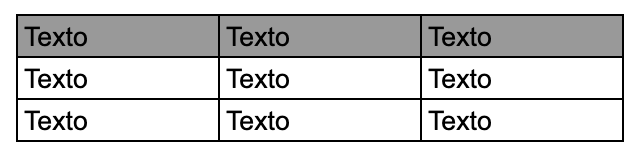
\includegraphics[height=3cm]{img/tablaejemplo.png} 
    \\ \scriptsize{Texto opcional al el pie de Tabla.}
    \label{img:referencia3}
\end{table}


\subsection{Usar plantilas}
\begin{minipage}[H]{0.49\textwidth}
    \begin{table}[H]
        \centering
        \caption{Tabla de referencia 2}
        \begin{tabular}{| l | c | r |} 
        \hline
            \textbf{Texto} & \textbf{Texto} & \textbf{Texto} \\ \hline
            Textoblabla    & Textoblabla   & Textoblabla \\ \hline
            Texto    & Texto   & Texto \\ \hline
        \end{tabular}
        \\ \scriptsize{Texto opcional al el pie de Tabla.}
    \end{table}
\end{minipage}
\begin{minipage}[H]{0.49\textwidth}
    \begin{table}[H]
        \centering
        \caption{Tabla de referencia 3}
        \begin{tabular}{l l l}
        \toprule
            \textbf{Texto} & \textbf{Texto} & \textbf{Texto} \\
            \midrule
            Textoblabla    & Textoblabla   & Textoblabla \\
            Texto    & Texto   & Texto \\
            \bottomrule
        \end{tabular}
        \\ \textit{\scriptsize{Texto opcional al el pie de Tabla.}}
    \end{table}
\end{minipage}